\documentclass[a4paper]{article} % Specify A4 paper

% Optional packages
\usepackage[utf8]{inputenc} % Allows UTF-8 input
\usepackage[T1]{fontenc}    % Selects font encodings
\usepackage{amsmath}        % For mathematical formulas
\usepackage{graphicx}       % To include images
\usepackage[ngerman]{babel} % German language support
\usepackage{geometry}       % For page layout adjustments
\usepackage{lipsum}         % For generating dummy text to fill pages
\usepackage{blindtext}      % Another package for dummy text

% Adjust page margins if needed (optional, default article margins are usually fine)
% \geometry{a4paper, margin=2.5cm}

% Document information
\title{Dokumentation zur Pipeline-Architektur}
\author{Ihr Name / Projektgruppe}
\date{\today}

\begin{document}

\maketitle % Displays title, author, and date
\tableofcontents % Add a table of contents
\newpage

\section{Praktische Umsetzung: Beispiel einer Datenverarbeitungs-Pipeline}
\subsection{Gesamtarchitektur}
Im folgenden Beispiel soll auf Basis der Pipeline-Architektur eine einfache Datenverarbeitungs-Pipeline beschrieben werden. Mit dieser Pipeline sollen Sensordaten geladen, verarbeitet und gespeichert werden. Die Pipeline besteht dabei aus mehreren Segmenten wobei der Ladepunkt der Datei als Startpunkt dient.
Die Architektur ist in Abbildung \ref{fig:architektur} dargestellt. Die einzelnen Stufen sind in der Abbildung nummeriert.
Die Pipeline besteht aus den folgenden Stufen:
\begin{enumerate}
    \item \textbf{Datenerfassung:} Sammeln von Rohdaten von Sensoren.
    \item \textbf{Vorverarbeitung:} Bereinigen und Filtern der Rohdaten.
    \item \textbf{Anreicherung:} Hinzufügen von Kontextinformationen (z.B. Zeitstempel, Standort).
    \item \textbf{Analyse:} Durchführung spezifischer Berechnungen oder Mustererkennung.
    \item \textbf{Speicherung/Ausgabe:} Persistieren der Ergebnisse oder Weiterleitung an andere Systeme.
\end{enumerate}

\subsection{Pipeline Wrapper Klasse}
Für die Ausführung der Pipeline sind verschiedene Ansätze möglich. Zum einen kann die Pipeline als Code direkt vom Entwickler definiert werden, als Konfigurationsdatei hinterlegt und bei Programmstart geladen werden oder als Wrapper-Klasse implementiert werden.

Das Laden durch eine Konfigurationsdatei hat den Vorteil dass der Aufbau der Pipeline dynamisch nach den spezifischen Anforderungen angepasst werden kann. Der Nachteil dieser Technik ist ein größerer Aufwand bei der Implementierung und Testen des Codes.

Die direkte Code Implementierung und der Ansatz via Wrapper-Klasse sind dabei sehr ähnlich in bezug darauf das der Entwickler die Pipeline direkt implementiert. Der Vorteil der Wrapper-Klasse ist, dass die Handhabung der Einzelnen Schritte der Pipeline in einer getrennten Klasse gehandhabt wird. Dadurch ist der Code gekapselt wodurch Code Änderungen und Bugfixes einfacher durchgeführt werden können. Darüber hinaus ist die Datei in welcher die Pipeline definiert wird aufgeräumter da die Handhabung ausgelagert ist. Nachteil dieser Herangehensweise ist, dass bei Projekten bei welchen die einzelnen Pipeline Schritte sich stark unterscheiden dieses Konzept nur schwer umsetzbar ist.

Da es sich bei diesem Beispiel nur um eine Einfache Lade und Verarbeitungs-Pipeline handelt, wird die Wrapper-Klasse verwendet. Diese ist in Abbildung \ref{fig:wrapper} dargestellt.

\begin{figure}[htbp] % h: here, t: top, b: bottom, p: page of floats
    \centering % Center the image
    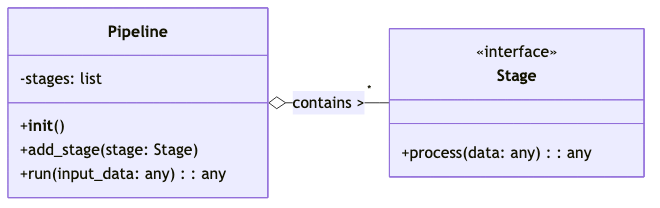
\includegraphics[width=0.8\textwidth]{img/wrapper.png} % Include the image, adjust width as needed
    \caption{Diagramm der Pipeline Wrapper Klasse} % Add a caption
    \label{fig:wrapper} % Add a label for referencing
\end{figure}

Die Pipeline Klasse stellt dabei funktionen zum Hinzufügen von Stufen sowie zum Ausführen der Pipeline auf Basis von Eingabedaten aus. Darüber hinaus verfügt die über eine Init Funktion zum erzeugen notwendiger Variablen. Die Einzelnen Stufen der Pipeline sind dabei durch die Abstrakte Klasse \texttt{PipelineStep} definiert. Diese Klasse definiert notwendige Funktionalitäten zum Ausführen einer Stufe. Dabei wird in der Abstrakten Klasse diese Funktionen nicht definiert sondern ausschließlich die Deklaration. Für die Implementierung sind die Kinderklassen zuständig. Dadurch ist sichergestellt, dass alle an die Pipeline übergebenen Stufen die benötigten Funktionsaufrufe implementieren.

\begin{verbatim}
def add_stage(self, stage:Stage):
    if(not issubclass(stage, Stage)):
        raise TypeError("stage must be an instance of Stage")
\end{verbatim}\

Diese Sicherung wird in Python durch das Prüfen des Klassentyps (issubclass) sichergestellt. Wird eine Klasse übergeben welche keine Subklasse von Stage ist wird ein TypeError geworfen. Dies geschieht bei issubclass selbst bei einer erzeugten Instanz von Stage selbst.

\subsection{Factory Pattern}
Ein beliebtes Architekturpattern welches sehr gut mit der Pipeline-Architektur zusammenarbeitet ist das Factory Pattern.

Das Factory Pattern ermöglicht eine Entkoppelung des Hauptcodes von der Ausführung eines spezifischen Code blocks. Dabei entscheidet die Factory abhängig von den übergebenen Parametern, welche auszuführende Klasse erzeugt werden soll. Dies hat den Vorteil dass der Entscheidungscode von dem Ausführenden Code getrennt ist. In unserem Beispiel wird dies unter anderem bei der Funktion zum Auslesen der Sensordateien verwendet. Hierbei übergibt der vorherige Schritt den Dateipfad welcher geladen werden soll. Die Factory entscheidet dann anhand des Dateiformats, welche Klasse zum Auslesen der Datei verwendet werden soll.

\begin{figure}[htbp] % h: here, t: top, b: bottom, p: page of floats
    \centering % Center the image
    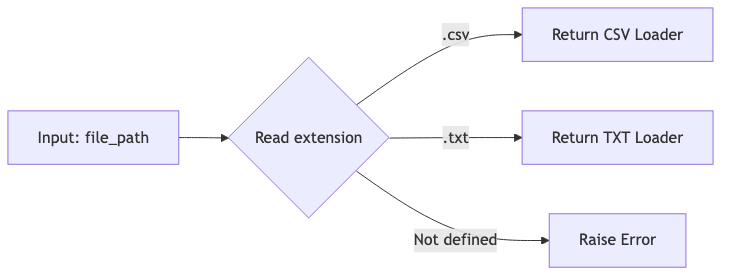
\includegraphics[width=0.8\textwidth]{img/LoaderFactory.png} % Include the image, adjust width as needed
    \caption{Diagramm der Pipeline Wrapper Klasse} % Add a caption
    \label{fig:loaderFactory} % Add a label for referencing
\end{figure}

\subsection{Implementierungsdetails Stufe 3: Anreicherung}
Beschreibung der Implementierung der dritten Stufe.
\blindtext[2]
\lipsum[13-14]

\subsection{Implementierungsdetails Stufe 4: Analyse}
Beschreibung der Implementierung der vierten Stufe.
\blindtext[2]
\lipsum[15-16]

\subsection{Implementierungsdetails Stufe 5: Speicherung/Ausgabe}
Beschreibung der Implementierung der fünften Stufe.
\blindtext[2]
\lipsum[17-18]


\section{Herausforderungen und Lösungsansätze}
Bei der Implementierung von Pipelines können verschiedene Herausforderungen auftreten.
\subsection{Fehlerbehandlung}
Wie werden Fehler in einzelnen Stufen behandelt? Weitergabe? Logging? Abbruch der Pipeline?
\lipsum[19-21]

\subsection{Monitoring und Debugging}
Wie wird der Zustand der Pipeline und der einzelnen Stufen überwacht? Wie können Probleme diagnostiziert werden?
\blindtext[3]
\lipsum[22]

\subsection{Lastverteilung und Skalierung}
Wie kann sichergestellt werden, dass keine Stufe zum Flaschenhals wird? Wie können einzelne Stufen bei Bedarf skaliert werden?
\lipsum[23-25]
\blindtext[2]


\section{Schlussfolgerung}
Zusammenfassend lässt sich sagen, dass Pipeline-Architekturen ein mächtiges Werkzeug für die Strukturierung von sequenziellen Verarbeitungsprozessen sind. Sie fördern Modularität, Parallelität und Wiederverwendbarkeit. Die Wahl der richtigen Granularität der Stufen, das Management von Puffern und eine robuste Fehlerbehandlung sind entscheidend für den Erfolg. Trotz der potenziellen Komplexität und Latenz bieten sie signifikante Vorteile für viele Anwendungsfälle, insbesondere in der Datenverarbeitung.
\lipsum[26-28]
\blindtext

\end{document}